\section{Ap\'endice: Framework de Benchmarking} \label{casos_de_prueba}

\subsubsection{Algoritmo exacto para la resolucion de CACM}

Se realiz\'o una experimentaci\'on para ver el comportamiento del algoritmo. Como se describi\'o en la secci\'on de complejidad (\ref{exacto:complejidad}), los grafos completos $K_n$ son los que van a requerir de una mayor cantidad de operaciones,
por lo que se generaron grafos $K_n$, con un $n$ fijo pero con los valore $\omega_1$ y $\omega_2$ aleatorios y un valor aleatorio para la cota $K$.
Para cada valor de $n$, se crearon varios grafos diferentes, y se midi\'o el tiempo promediado en 5 ejecuciones de cuanto tardaba el programa en encontrar o no la soluci\'on para cada un de esos grafos.

Se plasmaron \'estos tiempos en un gr\'afico y se calculo el promedio entre los diferentes grafos para un mismo $n$. Tambi\'en se grafic\'o el cociente entre el tiempo que se tard\'o y $n!$.

El programa logr\'o encontrar r\'apidamente soluciones, pero llegando a los $K_{16}$ se not\'o que creci\'o bastante el tiempo de ejecuci\'on y ya para el $K_{17}$ como tardaba m\'as de media hora se decidi\'o parar la prueba.

\subsubsection{Gr\'aficos}
A continuaci\'on se adjuntan los gr\'aficos del tiempo de ejecuci\'on:

Gr\'afico para grafos desde $K_5$ a $K_{16}$, cada punto azul representa una ejecuci\'on de un grafo en particular, y la l\'inea roja es el promedio entre los grafos del mismo $n$
\begin{center}
	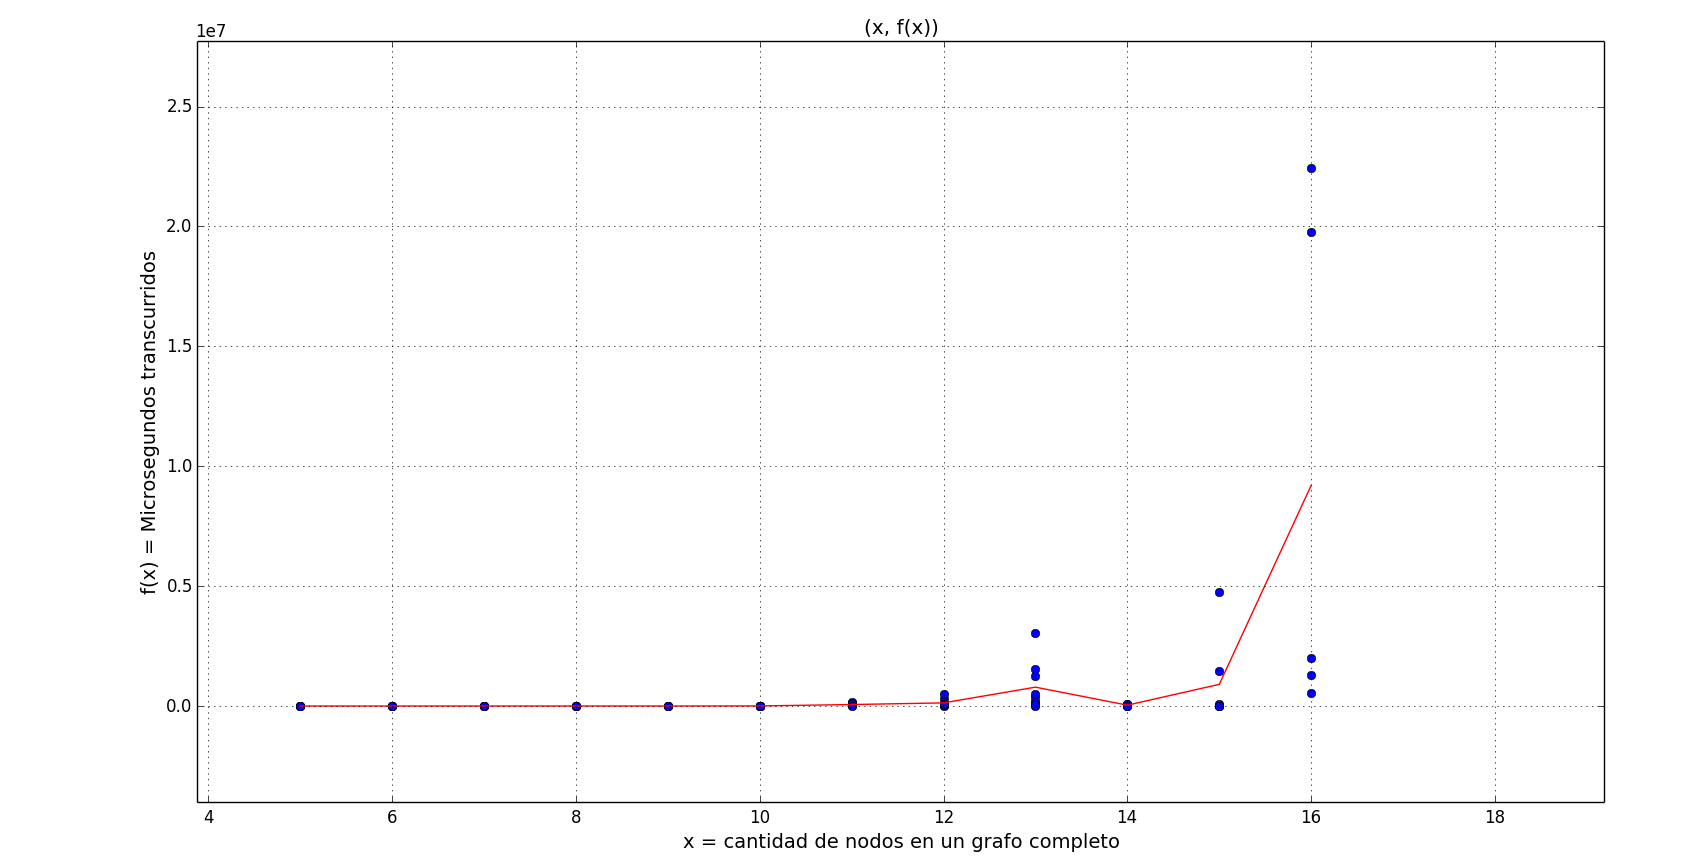
\includegraphics[scale=0.41]{img/exacto/fx_n_todo.png}
\end{center}

Dado que el tiempo crece demaciado r\'apido, tal como se esperaba, se dividi\'o el gr\'afico anterior para que se pueda apreciar mejor como fue creciendo:
\begin{center}
	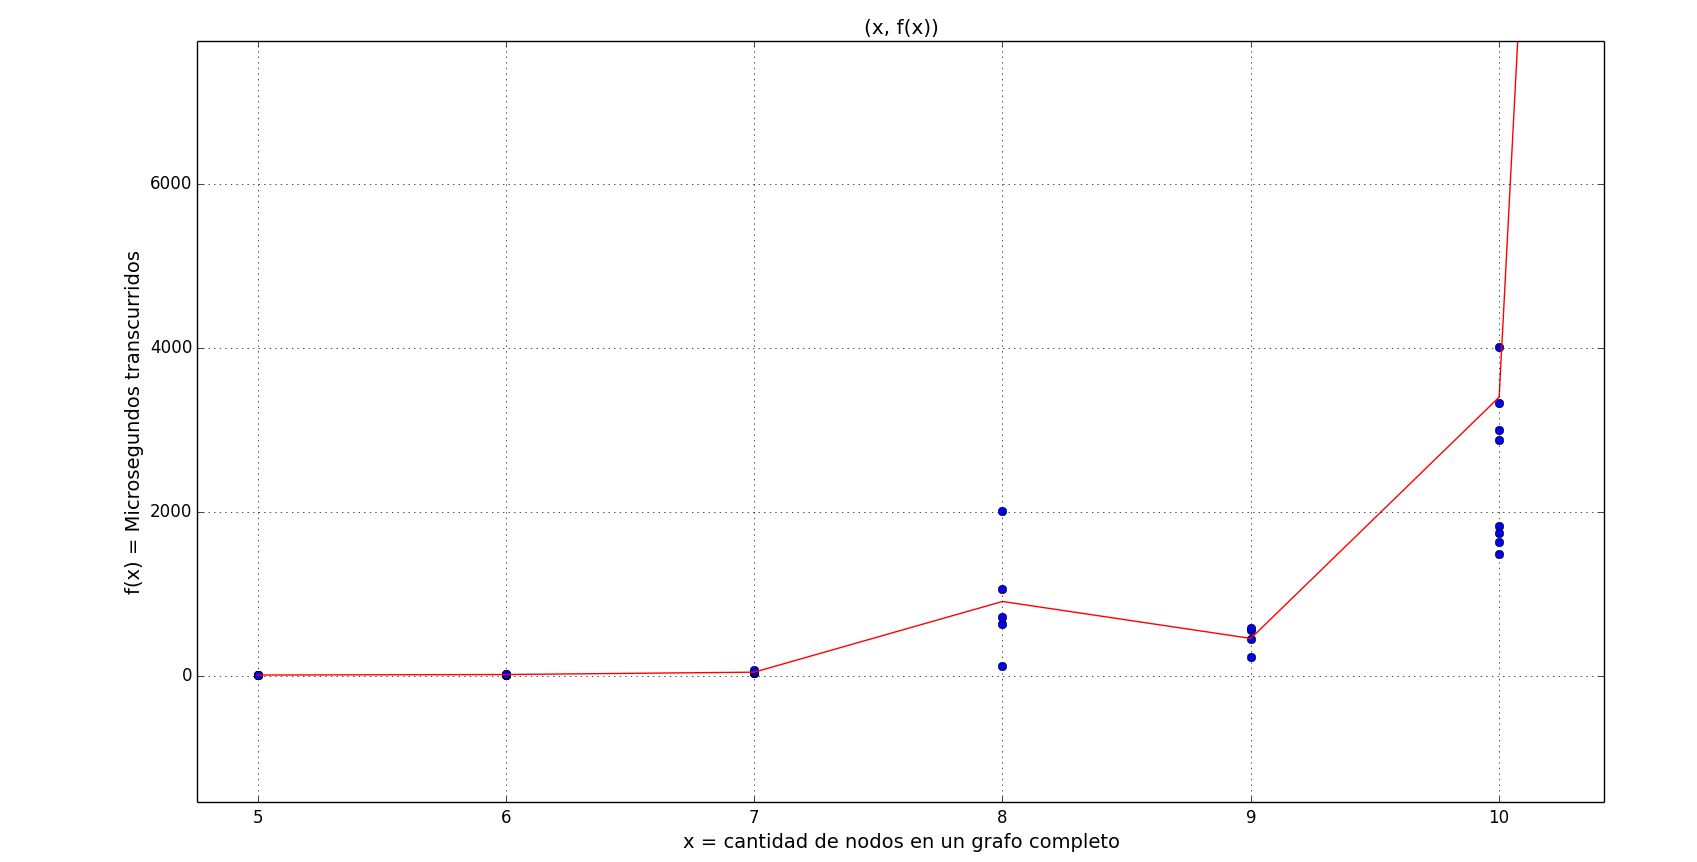
\includegraphics[scale=0.41]{img/exacto/fx_n_5_10.png}
\end{center}

\begin{center}
	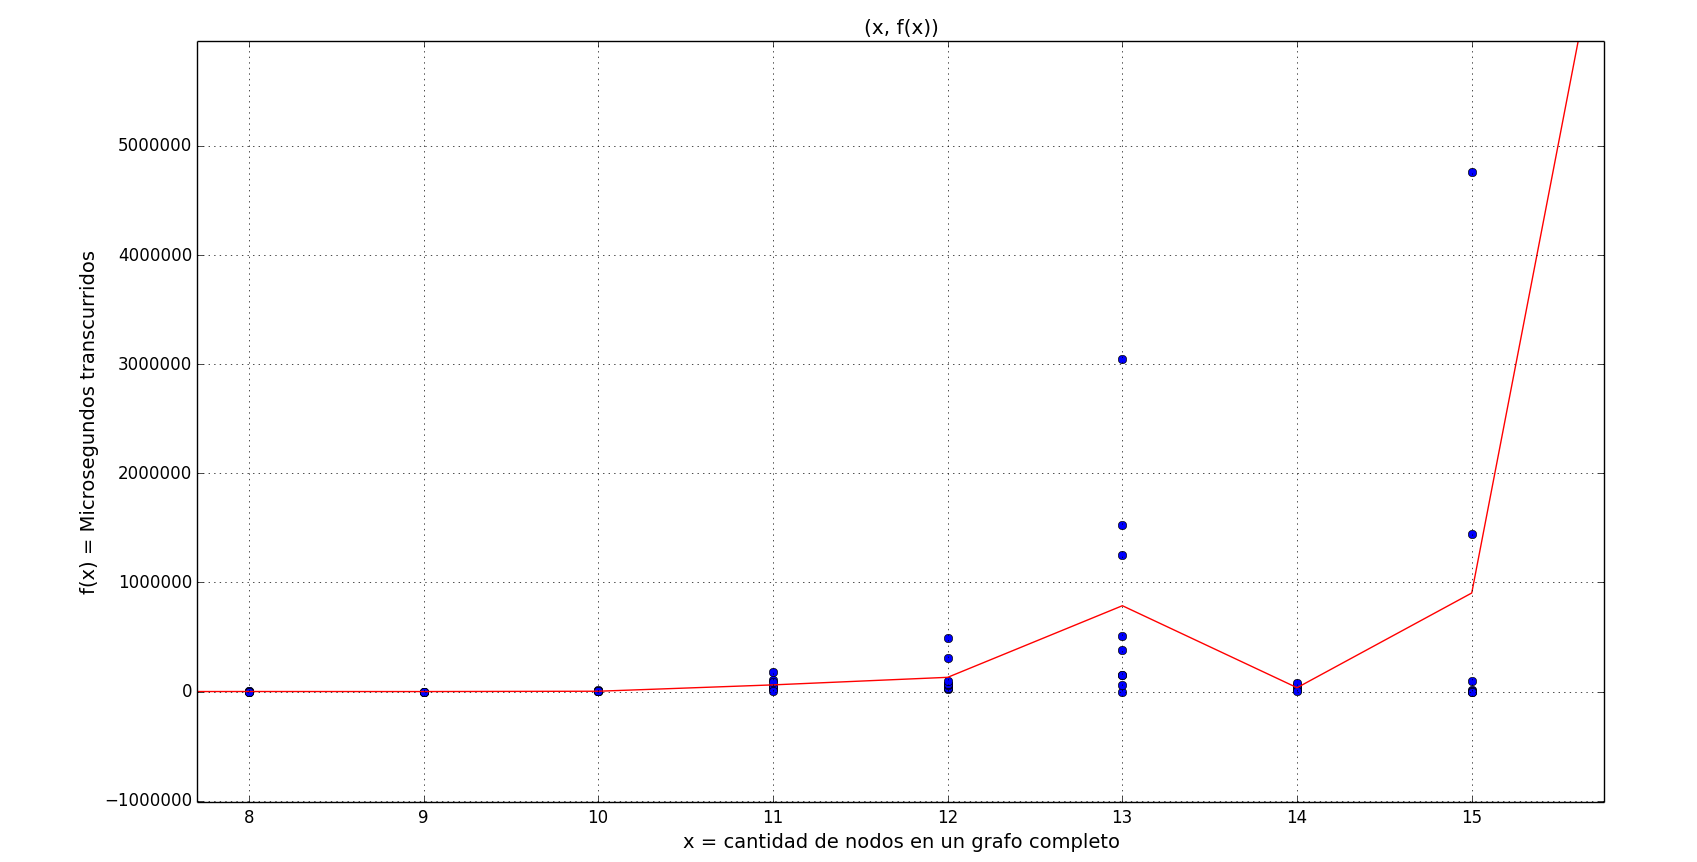
\includegraphics[scale=0.41]{img/exacto/fx_n_8_15.png}
\end{center}

\begin{center}
	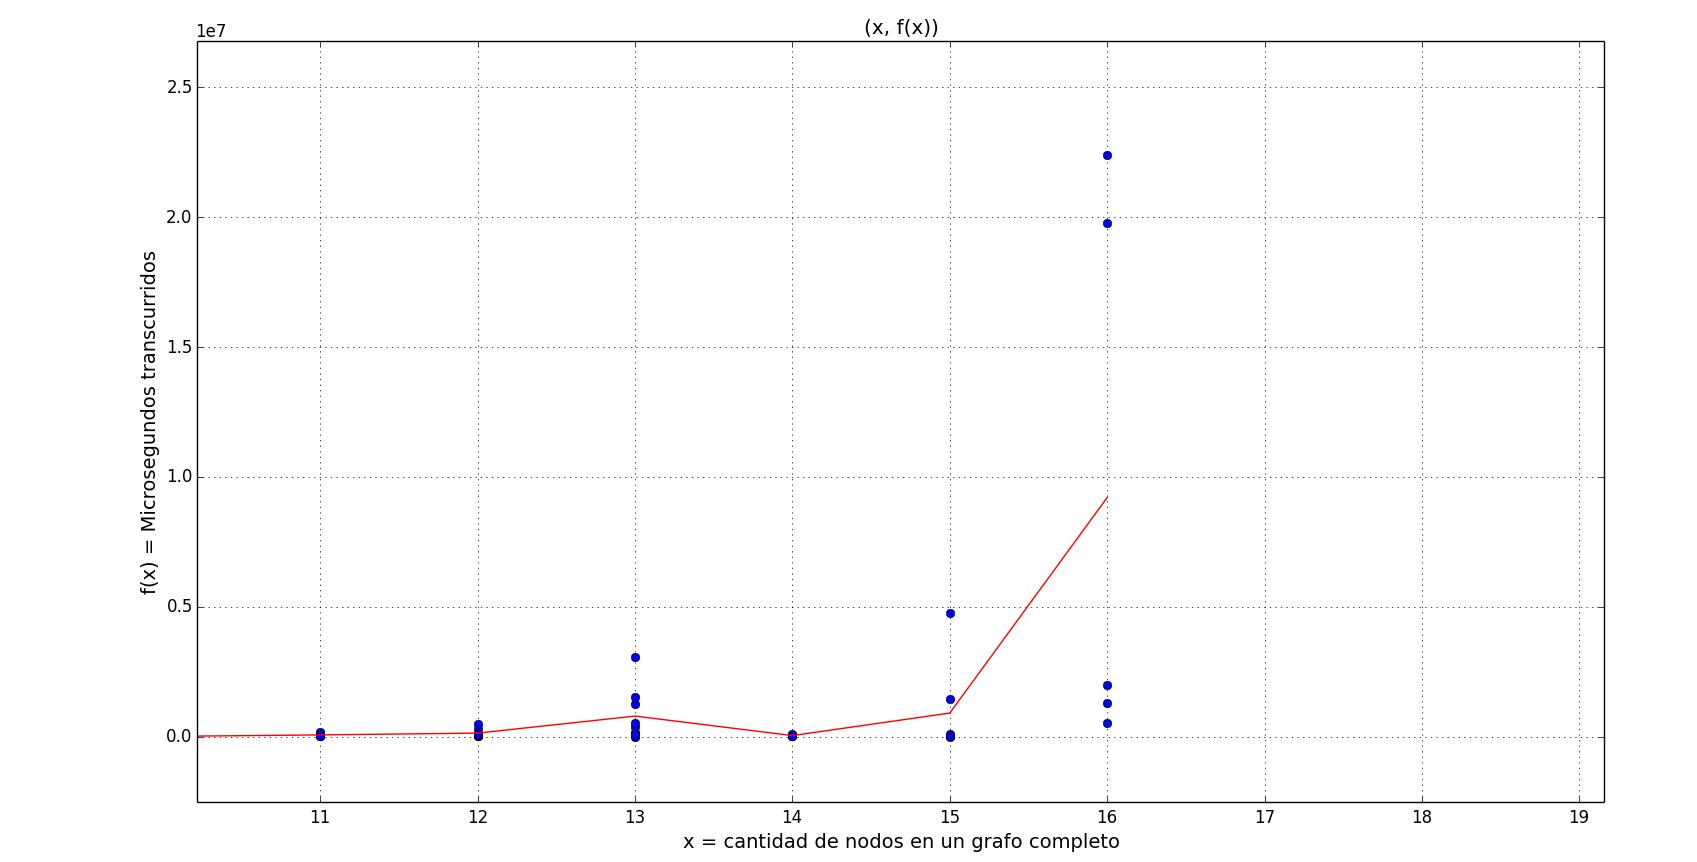
\includegraphics[scale=0.41]{img/exacto/fx_n_11_16.png}
\end{center}

Y luego se realiz\'o el cociente contra $n!$, que es la complejidad esperada. Se puede observar que el gr\'afico parece decrecer, pero s\'olo tenemos pocos valores que pudimos graficar.
\begin{center}
	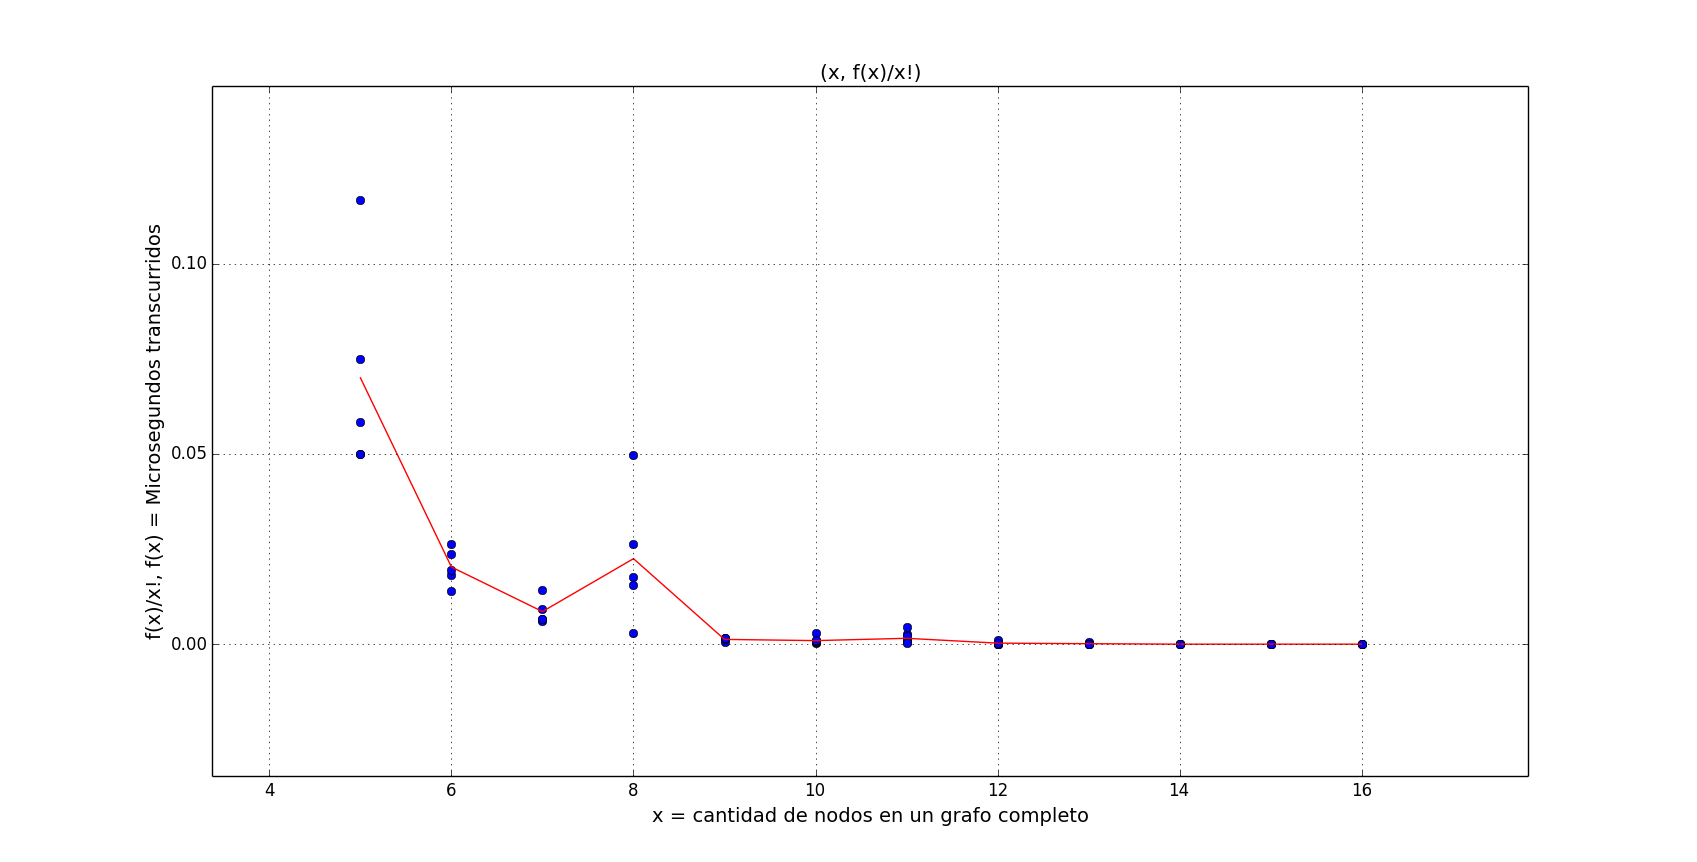
\includegraphics[scale=0.41]{img/exacto/fact_n.png}
\end{center}

Se dividi\'o el gr\'afico anterior para que se pueda apreciar mejor los valores:
\begin{center}
	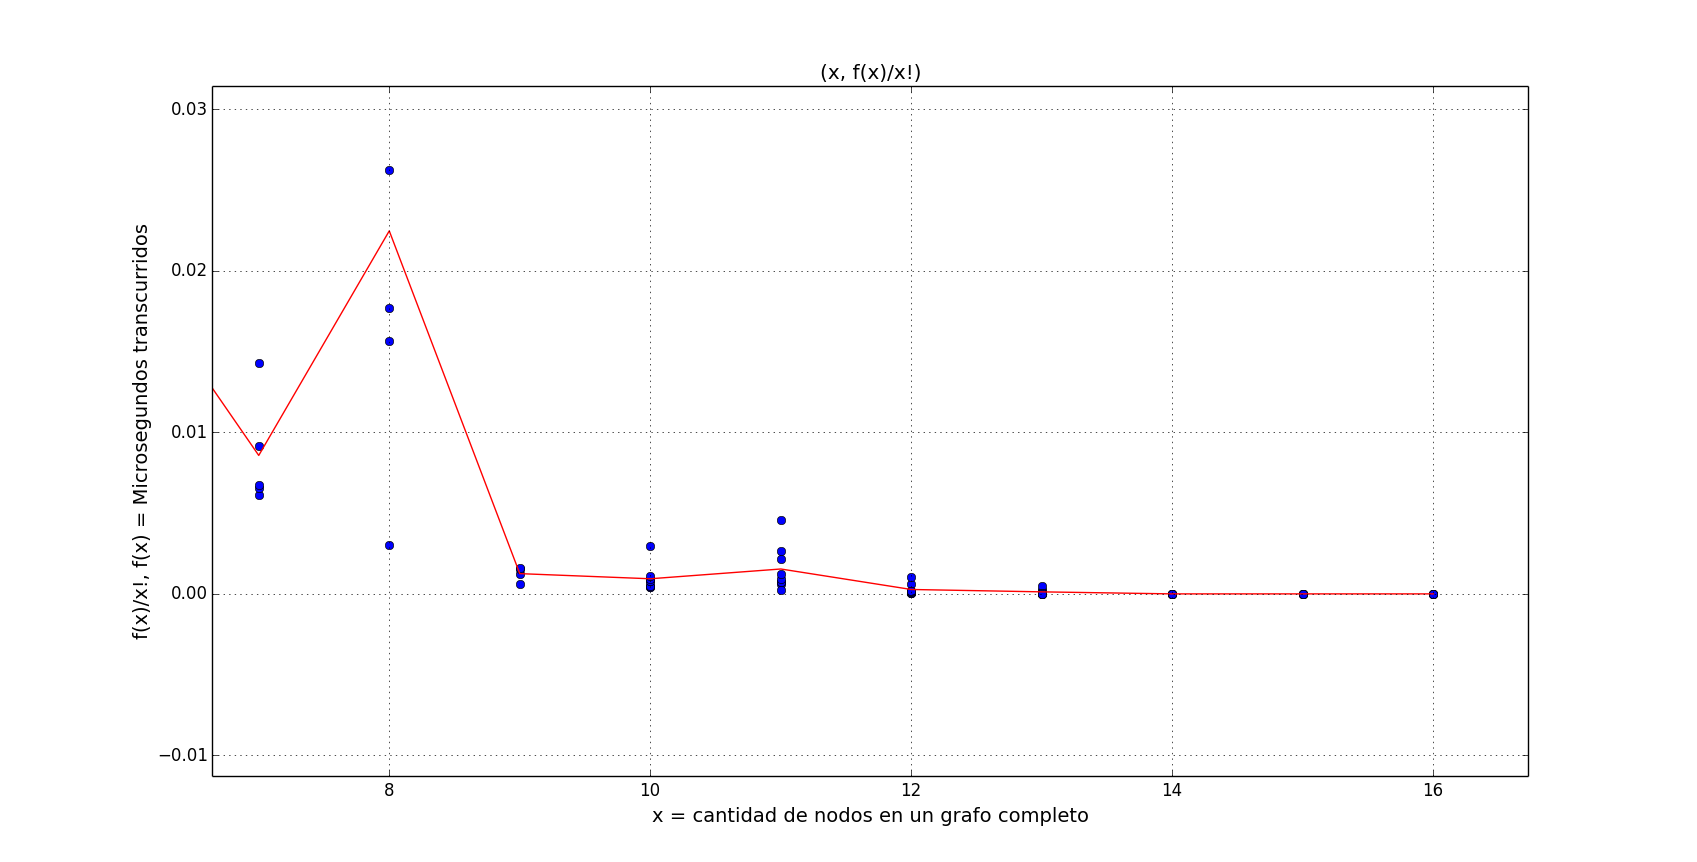
\includegraphics[scale=0.41]{img/exacto/fact_n_8_16.png}
\end{center}

\begin{center}
	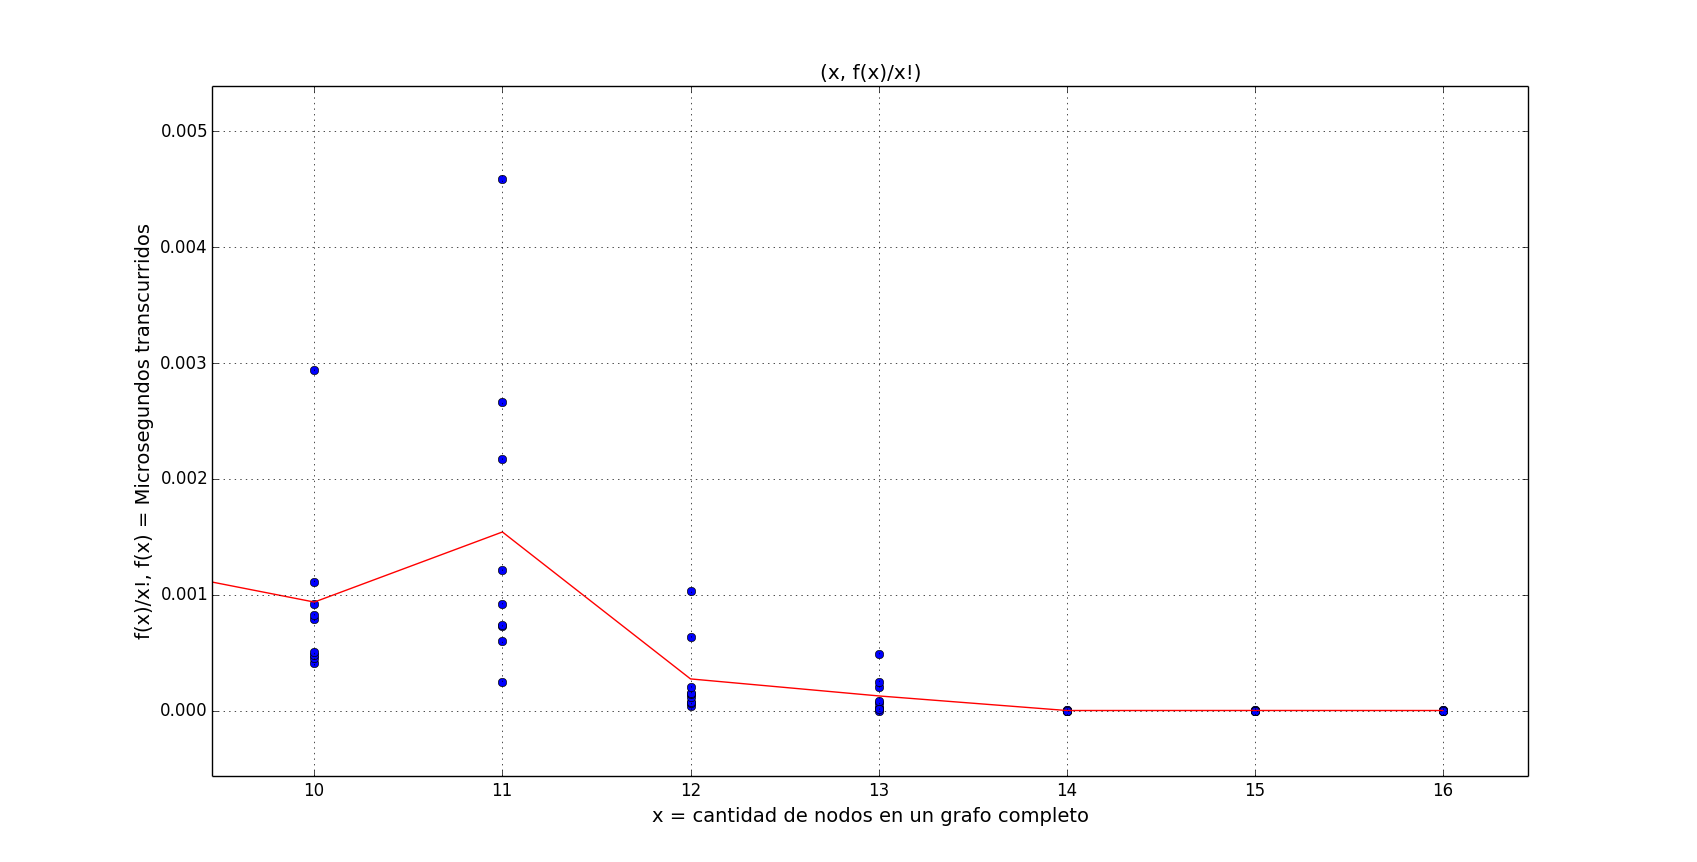
\includegraphics[scale=0.41]{img/exacto/fact_n_10_16.png}
\end{center}

\subsubsection{Concluciones}
Dada la complejidad del algoritmo, fueron pocos los tama\~nos de entrada que se pudieron medir, pero es el resultado que se esperaba.

Se puede ver que si bien tiende a crecer el tiempo de ejecucion, muchas veces distintos grafos de un mismo $n$ tuvieron tiempos muy diferentes de ejecuci\'on, not\'andose claramente en el $K_{16}$, donde 3 grafos tardaron menos de 5 segundos, pero otros 2 grafos tardaron 20 segundos o m\'as. \'Esto se puede deber a las distintas condiciones y podas del algoritmo para quedarse s\'olo con caminos v\'alidos y que no se pasen de la cota $K$ ni que superen una posible soluci\'on ya encontrada.

\subsubsection{Heur\'istica golosa}

En la experimentaci\'on de perfomance de la heur\'istica golosa utilizamos un generador de grafos aleatorios, hacemos variar la cantidad de nodos, con una cantidad de aristas fija. Sea $n$ la cantidad de nodos, es nuestra variable y probamos con $m = (n^2)/2$, es decir grafos completos, y luego con grafos densamente promedio, un n\'umero de aristas promedio entre $n-1$ (\'arbos) y un grafo completo ($ m = (n - 1 + (n^2)/2) /2 $)

\begin{center}
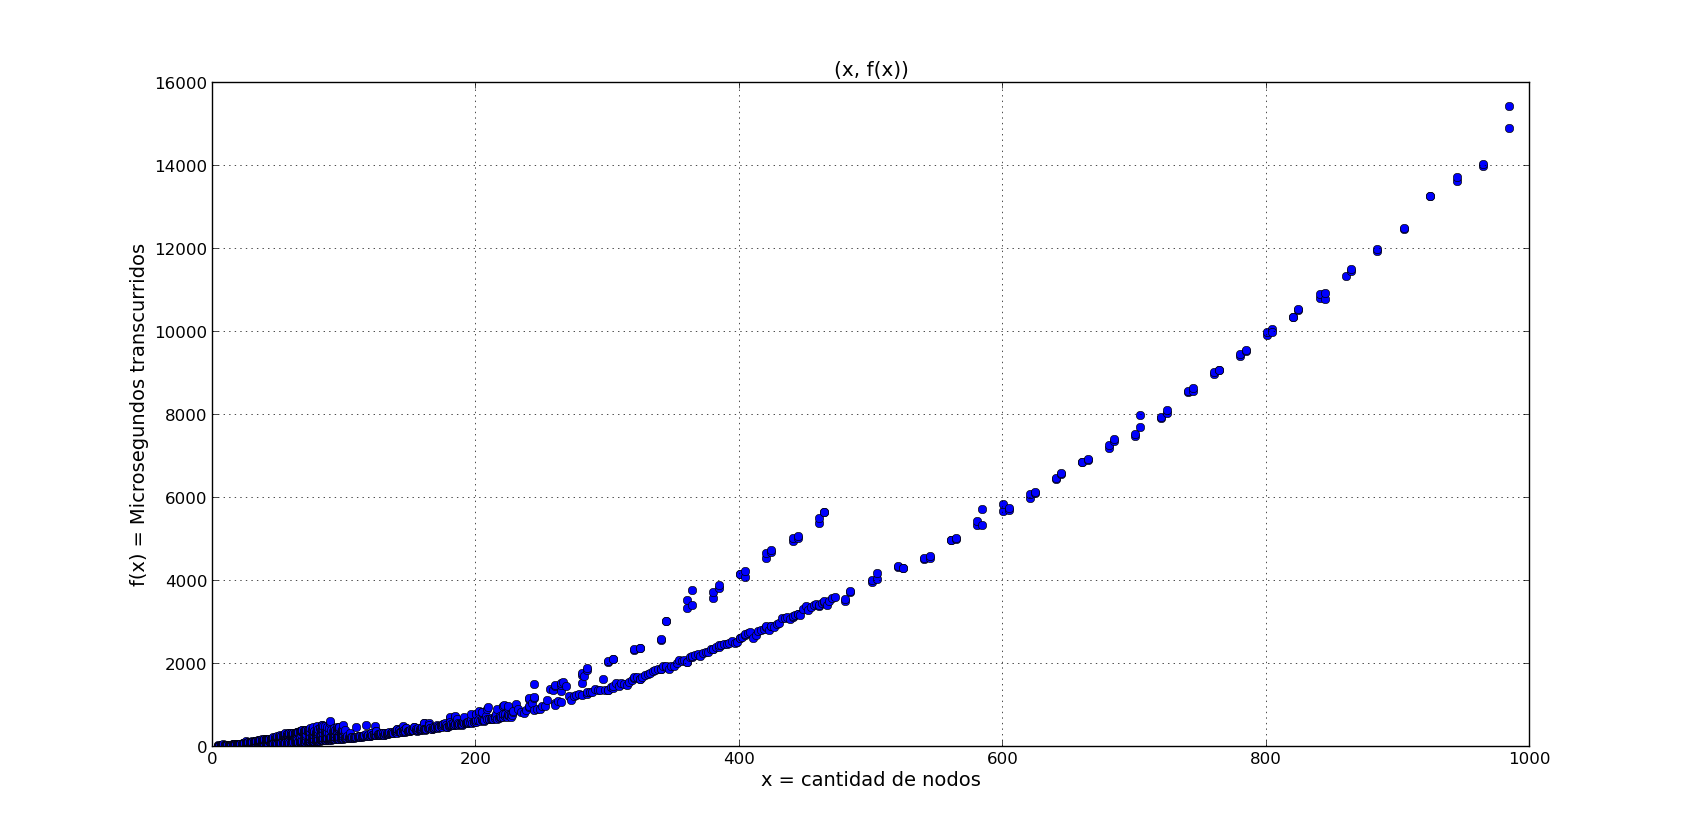
\includegraphics[scale=0.45]{img/golosa_fx.png}
\end{center}
\vspace{2mm}

Se puede apreciar una curva creciente con concavidad positiva. La curva de mayor valor que corta en 600 representa los valores de los grafos completos, que tuvimos que detener por razones de tiempo de c\'omputo. Vamos a dividir los resultados por $n^2$ y verificar que el resultado sea una curva constante.


\begin{center}
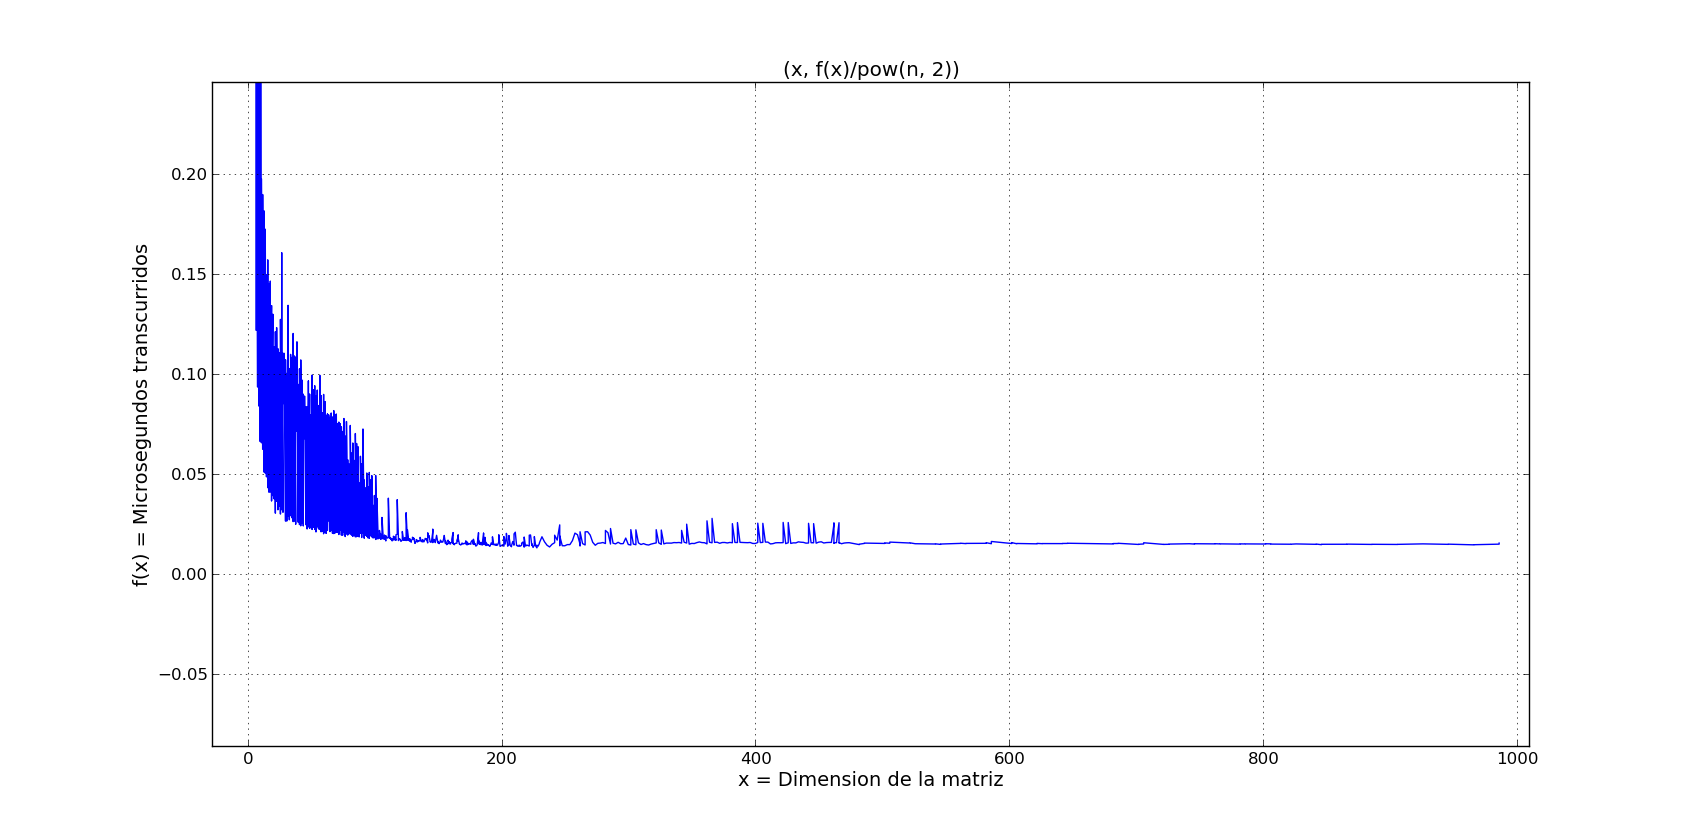
\includegraphics[scale=0.450]{img/golosa_fx2.png}
\end{center}
\vspace{2mm}

Puede apreciarse efectivamente una curva constante.
